\chapter{Fetch Stage}

We are ready to build our fetch unit.  To do this, we will make one more module, our instruction memory.  Then we will make a module to assemble all of our units together.


\section{Instruction Memory Module}
The instructions are stored in memory, and are accessed by using the address where they are stored.  You can think of memory like a giant hotel for our data.  Each piece of data is stored in a room (memory location), which we can find by its room number (memory address).  To get a piece of data stored in memory (like an instruction) we need to take its address, go to that location, and grab the data.  In Verilog, a bunch of memory locations that are accessed by an address is called an array.  Arrays in Verilog are declared like they are in C; the data type is specified, then the name, then the array size.  To store the instructions, we will need an array of 32-bit numbers (definitions.vh defines INSTR\_LEN as 32), which means the data type must be \verb2reg[`INSTR_LEN-1:0]2.  After the name is specified (imem in this case), we are going to use a parameter called SIZE to specify how many elements the array has: \verb2[SIZE-1:0]2.

The other interesting thing about this code is how to initialize the memory.  The default size of the memory is 1024 elements, so we do not want to initialize this memory element by element in the code.  Fortunately Verilog gives you two functions to do this automatically: \$readmemb and \$readmemh.  The last letter specifies the base (binary or hexadecimal) of the data in the file.  White space separates fields, but the underscore character is ignored and thus can be used to make the values in a number more readable.  The readmemb function will be used to read the file `IMEMFILE and store the bits in the imem array.  This is done one time on initialization.  Then, you can access that data in imem at any time after that.

`IMEMFILE is defined in definitions.vh, and I provide this file, which contains instructions.  However, you will need to update definitions.vh to point to your testfiles section rather than mine, or else it will look for mine and  not find the file.	

\Verilog{Instruction Memory}{code:instmem}{../code/1_fetch/instr_mem.v}

Starter code for the instruction memory module is given in Listing~\ref{code:instmem}.  There is only one line of code missing from this code.  Fill in the line of code inside the always block to complete the module.  Write a testbench and expected results table.  Verify that it operates correctly.  In order to confidently verify correct operation, you are required to create an Expected Results Table for your testbench and compare your simulation results with it.  Please show the instruction values in hexadecimal in the Expected Results Table and the Simulation Results.

\section{Fetch Stage}
Now we need to connect it together.  The components of our instruction fetch (sometimes called ifetch or just fetch) stage are shown in Figure~\ref{fig:fetch}.

\begin{wrapfigure}{L}{2in}
\caption{Instruction Fetch Stage.}\label{fig:fetch}
\begin{center}
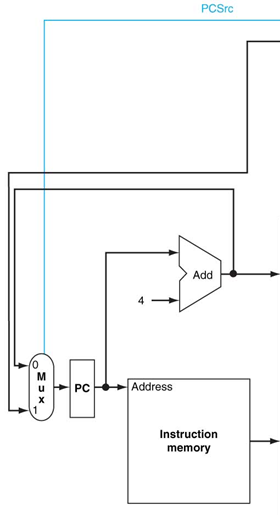
\includegraphics[width=2in]{../images/pipeline_fetch.png}
\end{center}
\end{wrapfigure}

Any wire (or reg) that comes into or goes out of the figure are input or output ports of the iFetch module.  In Figure~\ref{fig:fetch}, the blue wire is a control signal and comes ultimately from the control unit, which you will build in the decode stage.   Wires (or regs) that are completely contained in the figure are local to the iFetch module and are thus defined internally in the module.  The one exception to this is the current program counter (cur\_pc).  While there is no reason (at this point) that it must be output from the iFetch module, I strongly recommend making it an output so that it shows up on your simulation results, helping you to keep track of which instruction is currently executing.  Also, it will be required when we start pipelining our datapath in Lab 12.

While the input and output signals are easily identified by the diagram, you must also determine the size of each signal and whether it is a wire or reg.  When you look at the figure I cut from a figure in the book, note that I labeled every wire on the diagram in green.  For the sake of consistency and debugging, it is required that you use these names.  

IMPORTANT NOTE: Throughout your entire project, your signal names should follow the convention of the Freescale Semiconductor Verilog guide, which states that signal names should be all lower case, with words separated by an underscore.   

Once you have figured out all your connecting signals (wires and regs), you should identify the components you are going to use.  We have already created the modules, so now we just need to tell Verilog to instantiate them in the iFetch module and connect them together.  Create the iFetch module in a new file called iFetch.v in the code/1\_fetch directory.  

\section{Fetch Testbench}
Once you have made your connections, you should test the operation of the iFetch module by creating iFetch\_test.v.  You know you checked your individual modules, but there could be errors, or unexpected behavior when you put them together.  Sometimes weird timings between modules causes signals to be missed and such.  

Your testbench should create an instance of the iFetch module, set the inputs into the iFetch module, and verify that the correct outputs are produced. You should test both sequential operation (PC incrementing by 4) and branching.  When you test branching, keep in mind that my provided instruction file (instrData.data) only contains 14 instructions, so don't branch beyond the end of the file.

As we progress through this lab, you will learn how critical timing is.  Please look at the cur\_pc value and the instruction value and verify that the instruction that was fetched is the correct instruction, according to instrData.data and the current program counter.  Note that no instruction should be fetched in the first 5ns, as this is a half clock cycle and does not have a rising edge.  I have included a file called delay.v in code/0\_common.  It includes a module that inputs a clock signal and outputs a clock signal that is delay by some number of ns.  This will be useful when resolving timing issues.  Make sure to switch back and forth between sequential and branching to make sure that this works properly.

In order to confidently verify correct operation, you are required to create an Expected Results Table for your testbench and compare your simulation results with it.


\section{Your Assignment}
You are to:
\begin{enumerate}
\item Finish the instruction memory module.
\item Write a testbench for the instruction memory module.
\item Create an Expected Results Table for this testbench.
\item Verify the results of this testbench by comparing the Expected Results Table with the Simulation Results.
\item Finish the fetch stage.
\item Write a testbench for the fetch stage.
\item Create an Expected Results Table for this testbench.
\item Verify the results of this testbench by comparing the Expected Results Table with the Simulation Results.
\item Write up a lab report in \LaTeX\ following the lab format in \verb1LabN.tex1 and generate a pdf file.
\item Upload the pdf and all the Verilog files to Canvas.
\end{enumerate} 